\documentclass[../main.tex]{subfiles}

\SetKwProg{Fn}{Function}{:}{}

\begin{document}
\label{s_cellular}
The second implementation discussed in this paper is \textit{cellular automata} (CA). The CA approach, also known as majority dynamics, has originally been developed as a formal description of the Ising model~\cite{ising1925} and is extensively studied, see e.g.,~\cite{AbMo:15, Beetal16,  GaZe:18, MaRo:08, MoNeTa:13, Osetal:10, TaKiFu:96, WoOl:08}. More recently, it is also adopted in DLTs projects~\cite{nkn}.
One of the biggest advantages of the CA-based techniques over other consensus algorithms is the opportunity to achieve a very high level of parallelism.
This advantage alone is a sufficient incentive for deeper studies. Our proposed CA implementation brings the following novel key properties:
\begin{itemize}
    \item Every node acts as a cellular automaton~\cite{codd1968} that, in the presence of conflicts, changes its opinion only based on the state of its direct neighbors and always adopts the majority opinion. 
    \item The set of neighbors of a node does not change during one run of the consensus algorithm.
    In this case, the reorganization mentioned in Section~\ref{sec:peering} must only happen for different runs, i.e., different conflicts.
    \item When evaluating the opinions of neighbors, nodes will require a “proof” that includes the opinions of the neighbors' neighbors. This will allow nodes to monitor each others' behavior and prevents a node from lying independently of its neighbors.
    \item Misbehaving neighbors, i.e., neighbors that hold an opinion that is inconsistent with this proof, will be dropped immediately.
    This information is then also broadcasted to the network for other nodes to verify and mark that corresponding node as malicious and prevent future connection attempts.
\end{itemize}

At the beginning of each round, every node sends a ``heartbeat'' of its current status. 
This includes its signed current opinion, as well as the opinions of each of its neighbors from the previous round, each signed by the issuing node.
Since the previous opinions of the neighbors cannot be faked, every node receiving this heartbeat can validate that the current opinion is indeed correct and follows the rules of the consensus mechanism.

We formalize the above ideas in the consensus protocol described in the next subsection.

\SetKwFunction{FHeartbeat}{heartbeat}

\begin{algorithm}[h]
	\DontPrintSemicolon
			
	\Fn{\FHeartbeat{Node $i$, Round $m$}}{
		\ForEach{neighbor $j \in N_i$}{
			send opinion $X_{m}(i)$ to neighbor $j$\;
			\ForEach{$j' \in N_i\setminus \{j\}$}{
				send opinion $X_{m-1}(j')$ to neighbor $j$\;
		}}
	}
	\caption{Send heartbeat}
	\label{alg:heartbeat}
\end{algorithm}

\begin{algorithm}[h]
	\DontPrintSemicolon
			
	\ForEach{node $i$}{
		Send initial opinion $X_0(i)$ to neighbors $N_i$\;
	}
	\BlankLine
			
	\For{$m\gets 1$ \KwTo $M$}{
		\ForEach{node $i$}{
			\ForEach{neighbor $j \in N_i$}{
				\If{$X_{m-1}(j)$ is inconsistent wrt $X_{m'}(j')$ for $j' \in N_j, m' < m-1$}{
					\tcp{drop neighbor $j$}
					$N_i \gets N_i \setminus \{j\}$\;
				}
			}
			\uIf{node $i$ finalized}{
				$X_m(i) \gets X_{m-1}(i)$\;
				}\Else{
				\tcp{adopt majority opinion}
				$total \gets \sum_{\{j \in N_i\}} p(|N_j|)$\;
				\uIf{$\sum_{\{j \in N_i \mid X_{m-1}(j) = 0\}} p(|N_j|) > \frac{total}{2}$}{
					$X_m(i) \gets 0$\;
					}\uElseIf{$\sum_{\{j \in N_i \mid X_{m-1}(j) = 1\}} p(|N_j|) > \frac{total}{2}$}{
					$X_m(i) \gets 1$\;
					}\Else{
					$X_m(i) \gets \bot$ \tcp*{cancel all}
				}
			}
			\BlankLine
									
			\FHeartbeat{$i$, $m$}\;
			\BlankLine
									
			\If{opinion $X(i)$ did not change in the last $\ell$ rounds}{
				mark node $i$ finalized\;
			}
		}
	}
	\caption{Cellular consensus}
	\label{alg:cell}
\end{algorithm}

\paragraph{Model}

Suppose that there is a network composed of $n$ nodes, and these nodes need to come to a consensus on the value of a bit.
For clarity, we assume in the following that each node is directly connected to $k$ neighbors, through the autopeering mechanism described in Section~\ref{sec:peering}.
The set of neighbors of node~$i$ is denoted by $N_i$.
The autopeering mechanism is a key factor for the security of this approach, since a malicious node should not be able to select or influence its neighbors.

During each stage of the algorithm, each node holds an opinion on the value of the bit.
The opinion can be either $0$, $1$ or $\bot$, depending on whether the node prefers 0, 1 or none at all.
The opinion of node~$i$ in round~$m$ is denoted by~$X_m(i) \in \{0,1, \bot\}$. 
We further assume, that each node $i$ has the initial opinion $X_0(i) \in \{0,1\}$.

The protocol depends on the following parameters:
\begin{itemize}
	\item $k \in \mathbb{N}$, number of (initial) neighbors of each node.
	\item $M \in \mathbb{N}$, maximum number of rounds.
	\item $\ell \in \mathbb{N}$, the number of consecutive rounds with the same opinion after which it becomes final.
	\item $p : \{0,\dots,k\} \to \mathbb{R}_{\geq 0}$, monotonically increasing weight function that maps the number of neighbors to a weight. This penalizes nodes having fewer than $k$ neighbors.
\end{itemize}

\paragraph{Algorithm}

\begin{figure}%[H]
	\captionsetup[sub]{font=footnotesize}
	\centering
	\hfill
	\begin{subfigure}[b]{0.49\linewidth}
		
\includegraphics[width=\linewidth]{ca3}
		\caption{opinions ``collide'' (first nodes update opinion)}
	\end{subfigure}
	\begin{subfigure}[b]{0.49\linewidth}
		
\includegraphics[width=\linewidth]{ca4}
		\caption{opinions ``compete'' (nodes update their opinions)}
	\end{subfigure}
	\hfill
	\begin{subfigure}[b]{0.49\linewidth}
		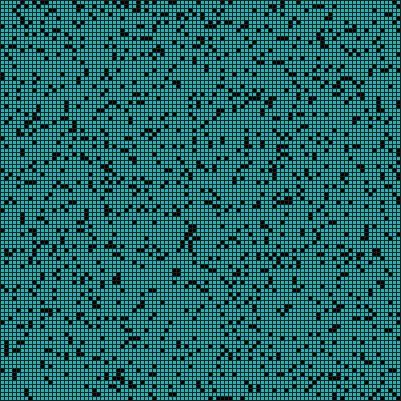
\includegraphics[width=\linewidth]{ca5}
		\caption{opinions ``compete'' (nodes update their opinions)}
	\end{subfigure}
	\hfill
	\begin{subfigure}[b]{0.49\linewidth}
		
\includegraphics[width=\linewidth]{ca6}
		\caption{a single opinion ``survives'' (network reaches consensus)}
	\end{subfigure}
	\caption{Visualization of the CA consensus process:
		Each square corresponds to a node connected to random neighbors.
		Initially, the two conflicting transactions are propagated through the network.
		Then, nodes are consistently adapting their opinions (0: red, 1: cyan, $\bot$: black) before eventually coming to consensus.}
	\label{fig:ca}
\end{figure}

Each node $i$ knows the opinions of its neighbors $j \in N_i$ as well as the opinions of all their neighbors $N_j$.
This is assured by a broadcasting step where all the opinions are signed in such a way that the originating nodes as well as broadcasting node are unforgeable.
This is formalized in Algorithm~\ref{alg:heartbeat}.

The consensus mechanism is a CA where a node uses the opinions of its neighbors to update its own state.
When the majority of neighbors support either 0 or 1, the node adopts that opinion.
If none of these opinions has a majority, it adopts $\bot$, i.e., none of them.
As long as we assume that the set~$N_i$ is known at least for all of its neighbors~$i$, any node can use these simple rules to validate whether the reported opinion of neighbor~$i$ is consistent with the opinions of all nodes in $N_i$.
The overall consensus mechanism is more formally illustrated in Algorithm~\ref{alg:cell} and an illustration of the CA process for an example scenario can be found in Fig.~\ref{fig:ca}.

\end{document}
